%%%%%%%%%%%%%%%%%%%%%%%%%%%%%%%%%%%%%%%%%%%%%%%%%%%%%%%%%%%%%%%%%%%%%%%%%%%

\documentclass[a4paper,oneside,12pt]{article}
\usepackage{mystyle}

\begin{document}

\title{\Large\bf Trigonometric functions}
\author{%%
  Minh Van Nguyen \\
  \url{mvngu@gmx.com}
}
\date{\today}
\maketitle

\noindent
By now, you should be familiar with the sine function $\sin x$ and the
cosine function $\cos x$, where $x$ is an angle in radians.  In this
document, you will further investigate properties of the sine and
cosine functions.

\begin{itemize}
\item Application: equations of parabolic motion for projectiles.
\end{itemize}


%%%%%%%%%%%%%%%%%%%%%%%%%%%%%%%%%%%%%%%%%%%%%%%%%%%%%%%%%%%%%%%%%%%%%%%%%%%

\section{Vertical shift of sine function}

\begin{figure}[!htbp]
\centering
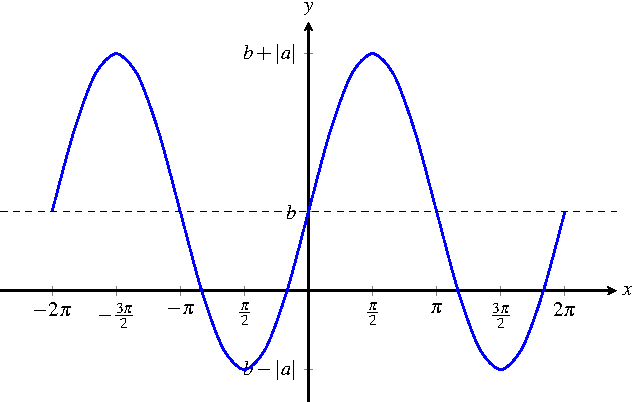
\includegraphics[scale=1.1]{image/13/a-sin-b.pdf}
\caption{%%
  A graph of the general sine function
  $f(x) = a \sin x + b$ from $x = -2\pi$ to $x = 2\pi$.  The midline
  of $f(x)$ is the dashed horizontal line $y = b$.  The amplitude of
  $f(x)$ is the absolute value $\absoluteValue{a}$.
}
\label{fig:trigonometric:general_sine}
\end{figure}

Let $a$ and $b$ be fixed real numbers and let $x$ be a real variable
that represents an angle in radians.  The sine function can be written
as
\[
f(x)
=
a \sin x + b
\]
which is graphed in \Figure{fig:trigonometric:general_sine}.  The
number $b$ is called the \emph{midline} of $f(x)$ and the absolute
value $\absoluteValue{a}$ is called the \emph{amplitude} of $f(x)$.
The amplitude $\absoluteValue{a}$ measures how high and how low the
value of the sine function $f(x)$ can be.  As you can see in
\Figure{fig:trigonometric:general_sine}, given the sine function
$f(x) = a \sin x + b$ the highest value of $f(x)$ is
$b + \absoluteValue{a}$, which is the value of the midline plut the
amplitude.  Furthermore, the lowest value of $f(x)$ is
$b - \absoluteValue{a}$, which is the value of the midline minus the
amplitude.  The number $b$ is the midline of the sine function $f(x)$
because the horizontal line $y = b$ is midway between the highest and
lowest values of $f(x)$.  In fact, if $h$ is the highest value of
$f(x)$ and $\ell$ is the lowest value of $f(x)$, then the value of the
midline is the average $\frac{h + \ell}{2}$.  If you draw the
horizontal line $y = b$ on a graph of $f(x)$~(e.g.~the dashed
horizontal line in \Figure{fig:trigonometric:general_sine}) you will
see that $f(x) = b$ whenever $a \sin x = 0$.  The above is summarised
in \Definition{def:trigonometric:sine_amplitude_and_midline}.

\begin{definition}
\label{def:trigonometric:sine_amplitude_and_midline}
\textbf{Amplitude and midline.}
Let $a$ and $b$ be fixed real numbers and let $x$ be a real variable.
Given a sine function of the form $f(x) = a \sin x + b$, the number
$\absoluteValue{a}$ is called the \emph{amplitude} of $f(x)$ and the
horizontal line $y = b$ is called the \emph{midline} of $f(x)$.
\end{definition}

\begin{figure}[!htbp]
\centering
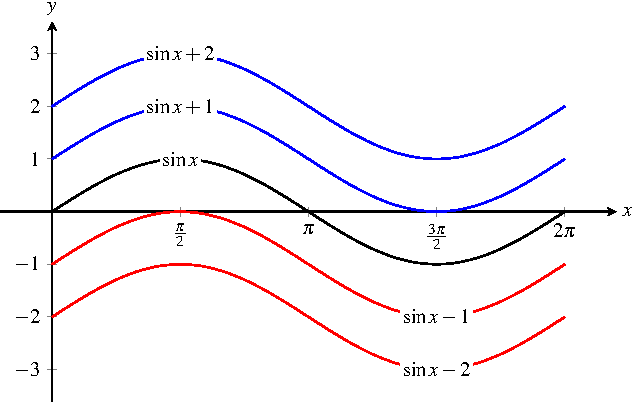
\includegraphics[scale=1.1]{image/13/sin-vertical-shift.pdf}
\caption{%%
  The value of the midline has the effect of vertically shifting the
  graph of the sine function.
}
\label{fig:trigonometric:sine_vertical_shift}
\end{figure}

How does the value of the midline affect the graph of the sine
function?  The value of the midline has the effect of shifting the
graph of the sine function vertically.  If the value of the midline is
positive, i.e.~$b > 0$, then the graph of the sine function will be
shifted upward.  However, if the value of the midline is negative,
i.e.~$b < 0$, then the graph of the sine function will be shifted
downward.  The vertical shift of the sine function is illustrated in
\Figure{fig:trigonometric:sine_vertical_shift}.

\begin{figure}[!htbp]
\centering
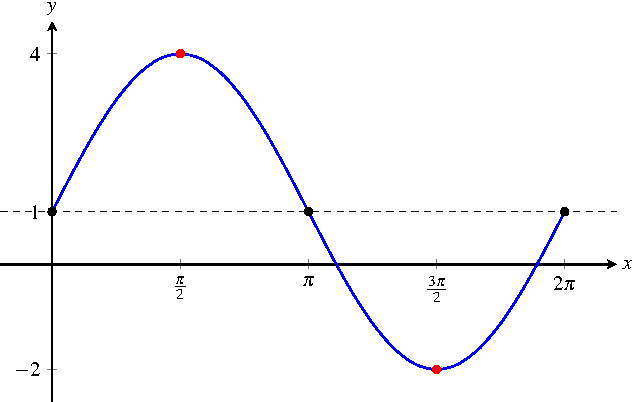
\includegraphics[scale=1.1]{image/13/3-sin-1.pdf}
\caption{%%
  A graph of the sine function $f(x) = 3 \sin x + 1$ from $x = 0$ to
  $x = 2\pi$.
}
\label{fig:trigonometric:sine_3_sin_1}
\end{figure}

\begin{example}
Consider the sine function $f(x) = 3 \sin x + 1$.  Determine the
midline and amplitude of $f(x)$.  Calculate the highest and lowest
values of the function.  Draw a graph of $f(x)$ from $x = 0$ to
$x = 2\pi$.
\end{example}

\begin{solution}
The first thing you should do is work out the midline and amplitude of
the function $f(x)$.  The midline of the function is $y = 1$.  The
amplitude is $3$.  The highest value of $f(x)$ is obtained by adding
the amplitude $3$ to the value of the midline.  Doing so gives you the
value $1 + 3 = 4$.  The lowest value of $f(x)$ is obtained by
subtracting the amplitude $3$ from the value of the midline.  Doing so
results in $1 - 3 = -2$.  Thus the highest value of $f(x)$ is $4$ and
the lowest value of $f(x)$ is $-2$.
\Figure{fig:trigonometric:sine_3_sin_1} shows the midline $y = 1$ as a
dashed horizontal line.

Next, determine all values of $x$ within the range
$0 \leq x \leq 2\pi$ such that the graph of $f(x)$ intersects the
midline.  This is equivalent to determining all values of $x$ such
that $\sin x = 0$.  The reason is that if $\sin x = 0$, then the
function $f(x) = 3 \sin x + 1$ simplifies to $f(x) = 1$, which is the
midline.  You know that $\sin x = 0$ when
$x = \triple{0}{\pi}{2\pi}$ and so you have
$f(0) = f(\pi) = f(2\pi) = 3 \times 0 + 1 = 1$.  In other words, the
graph of $f(x)$ intersects the midline $y = 1$ at the points
$\tuple{0}{1}$, $\tuple{\pi}{1}$, and $\tuple{2\pi}{1}$.
\Figure{fig:trigonometric:sine_3_sin_1} shows the points of
intersection as black dots.

Now determine the highest and lowest points of $f(x)$, where
$0 \leq x \leq 2\pi$.  To determine the highest point of $f(x)$, you
determine the highest value of $\sin x$.  You know that the highest
value of $\sin x$ is $1$, which occurs when $x = \frac{\pi}{2}$.  Then
the highest value of $f(x)$ is $f(\pi/2) = 3 \times 1 + 1 = 4$ so that
the highest point of $f(x)$ is $\tuple{\frac{\pi}{2}}{4}$.  Similarly,
the lowest value of $\sin x$ is $-1$, which occurs when
$x = \frac{3\pi}{2}$.  Then the lowest value of $f(x)$ is
$f(3\pi/2) = 3(-1) + 1 = -2$ so that the lowest point of $f(x)$ is
$\tuple{\frac{3\pi}{2}}{-2}$.  The highest and lowest points of $f(x)$
are shown in \Figure{fig:trigonometric:sine_3_sin_1} as red dots.

Finally, draw a wave through the above five points and you obtain the
graph in \Figure{fig:trigonometric:sine_3_sin_1}.
\end{solution}

\begin{exercise}
Consider the function $f(x) = 4 \sin x + 2$.  Determine the midline
and amplitude of $f(x)$.  Calculate the highest and lowest values of
the function.  Draw a graph of $f(x)$ from $x = 0$ to $x = 2\pi$.
\end{exercise}

\ifbool{showSolution}{
\begin{solution}
The midline of $f(x)$ is the horizontal line $y = 2$.  The amplitude
of $f(x)$ is $4$.  To obtain the highest value of $f(x)$, you add the
amplitude $4$ to the value of the midline and get $2 + 4 = 6$.  To
obtain the lowest value of $f(x)$, you subtract the amplitude $4$ from
the value of the midline and get $2 - 4 = -2$.  That is, the highest
and lowest values of $f(x)$ are $6$ and $-2$, respectively.

To graph $f(x)$ from $x = 0$ to $x = 2\pi$, you should first determine
those values of $x$ for which the graph of $f(x)$ intersects the
midline.  This is the same as determining all values of $x$ such that
$\sin x = 0$.  You know that $\sin 0 = \sin \pi = \sin 2\pi = 0$ so
that when $x = \triple{0}{\pi}{2\pi}$ you have
$f(0) = f(\pi) = f(2\pi) = 4 \times 0 + 2 = 2$.  Thus the graph of
$f(x)$ intersects the midline at the points $\tuple{0}{2}$,
$\tuple{\pi}{2}$, and $\tuple{2\pi}{2}$.

Next, you determine the highest and lowest points of $f(x)$ within the
range $0 \leq x \leq 2\pi$.  You know that the highest value of
$\sin x$ is $1$, which occurs when $x = \frac{\pi}{2}$.  Substitute
the latter value into $f(x)$ and you obtain
%%
\begin{align*}
f(\pi/2)
&=
4 \sin \frac{\pi}{2} + 2 \\[4pt]
&=
4 \times 1 + 2 \\[4pt]
&=
6.
\end{align*}
%%
The lowest value of $\sin x$ is $-1$, which occurs when
$x = \frac{3\pi}{2}$.  Substitute the latter value into the function
$f(x)$ and simplify to obtain
%%
\begin{align*}
f(3\pi / 2)
&=
4 \sin \frac{3\pi}{2} + 2 \\[4pt]
&=
4 (-1) + 2 \\[4pt]
&=
-4 + 2 \\[4pt]
&=
-2.
\end{align*}
%%
In other words, the highest point of $f(x)$ is
$\tuple{\frac{\pi}{2}}{6}$ and the lowest point of $f(x)$ is
$\tuple{\frac{3\pi}{2}}{-2}$.

\begin{figure}[!htbp]
\centering
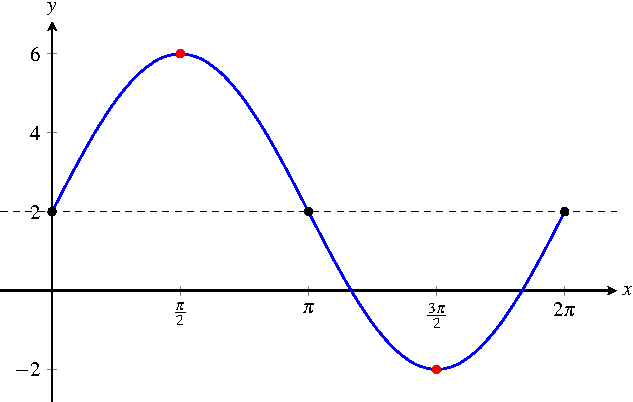
\includegraphics[scale=1.1]{image/13/4-sin-2.pdf}
\caption{%%
  A graph of the function $f(x) = 4 \sin x + 2$ from $x = 0$ to
  $x = 2\pi$.
}
\label{fig:trigonometric:4_sinx_2}
\end{figure}

Finally, draw a wave through the above points and you obtain the graph
shown in \Figure{fig:trigonometric:4_sinx_2}.  The black dots show the
points at which the graph of $f(x)$ intersects the midline $y = 2$.
The red dots show the highest and lowest points of $f(x)$.
\end{solution}
}{}

\begin{exercise}
Consider the function $f(x) = -2 \sin x + 6$.  Determine the midline
and amplitude of $f(x)$.  Calculate the highest and lowest values of
the function.  Draw a graph of $f(x)$ from $x = 0$ to $x = 2\pi$.
\end{exercise}

\ifbool{showSolution}{
\begin{solution}
The midline of the function $f(x)$ is $y = 6$ and the amplitude is
$\absoluteValue{-2} = 2$.  \Figure{fig:trigonometric:minus2_sin_6}
shows the midline as a dashed horizontal line.  The highest value of
$f(x)$ is obtained by adding the amplitude to the value of the
midline.  Then the required highest value is $6 + 2 = 8$.  Similarly,
the lowest value of $f(x)$ is obtained by subtracting the amplitude
from the value of the midline.  Thus the lowest value of $f(x)$ is
$6 - 2 = 4$.

\begin{figure}[!htbp]
\centering
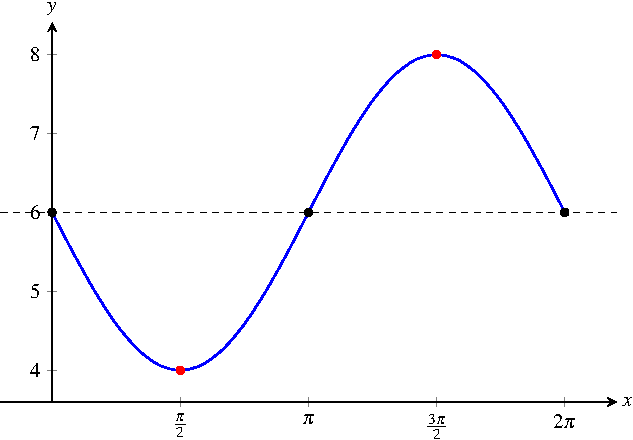
\includegraphics[scale=1.1]{image/13/minus2-sin-6.pdf}
\caption{%%
  A graph of the function $f(x) = -2 \sin x + 6$ from $x = 0$ to
  $x = 2\pi$.
}
\label{fig:trigonometric:minus2_sin_6}
\end{figure}

To draw a graph of the function $f(x)$ within the range
$0 \leq x \leq 2\pi$, you should first determine all points of $f(x)$
at which the graph of $f(x)$ intersects the midline.  This is the same
as determining all values of $x$ such that $\sin x = 0$.  You already
know that $\sin x = 0$ whenever $x = \triple{0}{\pi}{2\pi}$.  Then you
have $f(0) = f(\pi) = f(2\pi) = 6$.  In other words, the graph of
$f(x)$ intersects the midline at the points $\tuple{0}{6}$,
$\tuple{\pi}{6}$, and $\tuple{2\pi}{6}$.  The points of intersection
are shown in \Figure{fig:trigonometric:minus2_sin_6} as black dots.

Next, determine the highest and lowest points of $f(x)$.  Note that
the highest value of $\sin x$ is $1$, which occurs when
$x = \frac{\pi}{2}$.  Then $f(\pi/2) = -2 \times 1 + 6 = 4$, which is
the lowest value of $f(x)$.  That is, the lowest point of $f(x)$ is
$\tuple{\frac{\pi}{2}}{4}$.  Furthermore, the lowest value of $\sin x$
is $-1$, which occurs when $x = \frac{3\pi}{2}$.  Then you have
$f(3\pi/2) = -2 (-1) + 6 = 8$, which is the highest value of $f(x)$.
The highest point of $f(x)$ is $\tuple{\frac{3\pi}{2}}{8}$.  The
highest and lowest points are shown in
\Figure{fig:trigonometric:minus2_sin_6} as red dots.

Finally, draw a wave through the five points to obtain the graph shown
in \Figure{fig:trigonometric:minus2_sin_6}.
\end{solution}
}{}

\begin{figure}[!htbp]
\centering
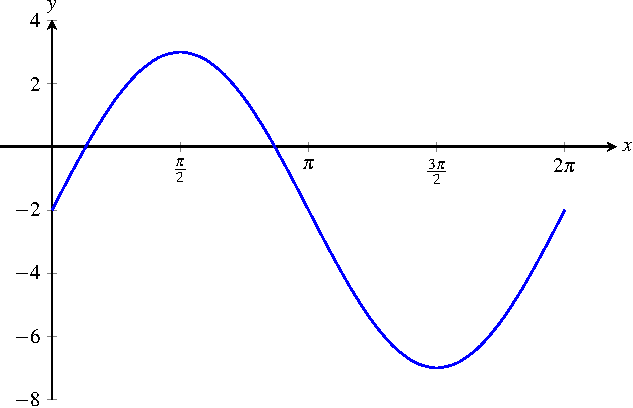
\includegraphics[scale=1.1]{image/13/5-sin-minus2.pdf}
\caption{%%
  A graph of a sine function of the form $f(x) = a \sin x + b$ from
  $x = 0$ to $x = 2\pi$.
}
\label{fig:trigonometric:5_sin_minus2}
\end{figure}

\begin{exercise}
\Figure{fig:trigonometric:5_sin_minus2} shows a graph of a sine
function that has a midline of $y = -2$.  The function has
$\tuple{\frac{\pi}{2}}{3}$ as one of its highest points.  If the
function is of the form $f(x) = a \sin x + b$, determine the values of
$a$ and $b$.
\end{exercise}

\ifbool{showSolution}{
\begin{solution}
Since the midline is $y = -2$, then $b = -2$.  The highest value of
$f(x)$ is obtained by adding the amplitude to the value of the
midline.  If the amplitude is $a$, then you have the equation
$-2 + a = 3$.  Solving the latter equation for $a$ yields
%%
\begin{align*}
a
&=
3 + 2 \\[4pt]
&=
5.
\end{align*}
%%
In other words, the amplitude is $a = 5$.  Therefore,
\Figure{fig:trigonometric:5_sin_minus2} shows a graph of the function
$f(x) = 5 \sin x - 2$.
\end{solution}
}{}

\begin{exercise}
A sine function $f(x) = a \sin x + b$ has
$\tuple{\frac{\pi}{2}}{\frac{15}{2}}$ and
$\tuple{\frac{3\pi}{2}}{-\frac{1}{2}}$ as some of its highest and
lowest points, respectively.  Determine the amplitude and midline of
$f(x)$.  Sketch a graph of $f(x)$ from $x = 0$ to $x = 2\pi$.
\end{exercise}

\ifbool{showSolution}{
\begin{solution}
Since $\frac{15}{2}$ is the highest value of $f(x)$ and $-\frac{1}{2}$
is the lowest value of $f(x)$, then the value of the midline is the
average of the highest and lowest values.  Thus the midline of $f(x)$
is
%%
\begin{align*}
y
&=
\frac{1}{2} \parenthesis*{\frac{15}{2} - \frac{1}{2}} \\[4pt]
&=
\frac{1}{2} \parenthesis*{\frac{15 - 1}{2}} \\[4pt]
&=
\frac{1}{2} \times 7 \\[4pt]
&=
\frac{7}{2}.
\end{align*}
%%
The amplitude of $f(x)$ is the difference between the highest value of
$f(x)$ and the value of the midline.  The amplitude is also the
difference between the value of the midline and the lowest value of
$f(x)$.  That is, the amplitude of $f(x)$ is
%%
\begin{align*}
a
&=
\frac{15}{2} - \frac{7}{2} \\[4pt]
&=
\frac{15 - 7}{2} \\[4pt]
&=
\frac{8}{2} \\[4pt]
&=
4.
\end{align*}
%%
Thus the function $f(x)$ can be written as
$f(x) = 4 \sin x + \frac{7}{2}$ and is graphed in
\Figure{fig:trigonometric:4_sin_7half}.

\begin{figure}[!htbp]
\centering
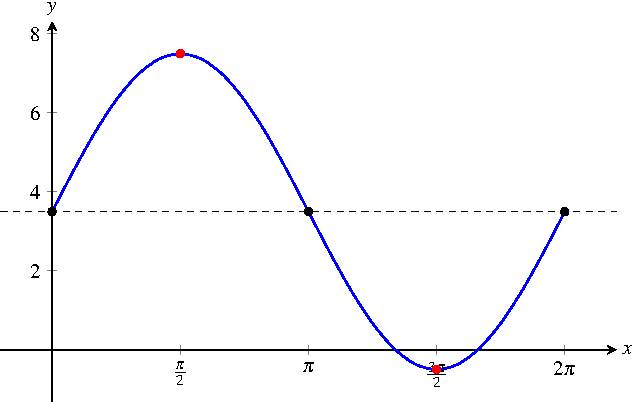
\includegraphics[scale=1.1]{image/13/4-sin-7half.pdf}
\caption{%%
  A graph of the function $f(x) = 4 \sin x + \frac{7}{2}$ from
  $x = 0$ to $x = 2\pi$.
}
\label{fig:trigonometric:4_sin_7half}
\end{figure}

\end{solution}
}{}

\begin{exercise}
Consider the function $f(x) = a \sin x$.  Graph the function when
$a = \triple{1}{\frac{3}{2}}{2}$.  Also graph the function when
$a = \triple{1}{\frac{1}{2}}{\frac{3}{4}}$.  Describe the effect of
the value of the amplitude on the graph of the sine function.
\end{exercise}

\ifbool{showSolution}{
\begin{solution}
\Figures{fig:trigonometric:sine_vertical_stretch}{fig:trigonometric:sine_vertical_compress}
show graphs of the function $f(x) = a \sin x$ when the values of the
amplitude are $a = \triple{1}{\frac{3}{2}}{2}$ and
$a = \triple{1}{\frac{3}{4}}{\frac{1}{2}}$.  As the figures show, when
the amplitude is $a > 1$, the graph of the sine function is stretched
in the vertical direction.  When the amplitude is $0 < a < 1$, the
graph of the sine function is compressed in the vertical direction.

\begin{figure}[!htbp]
\centering
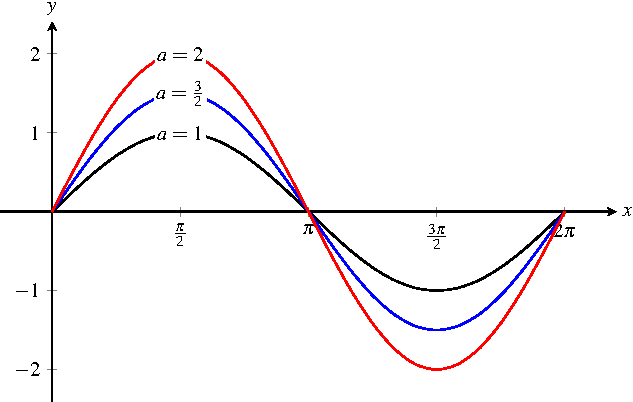
\includegraphics[scale=1.1]{image/13/sin-vertical-stretch.pdf}
\caption{%%
  Graphs of the function $f(x) = a \sin x$ for
  $a = \triple{1}{\frac{3}{2}}{2}$.
}
\label{fig:trigonometric:sine_vertical_stretch}
\end{figure}

\begin{figure}[!htbp]
\centering
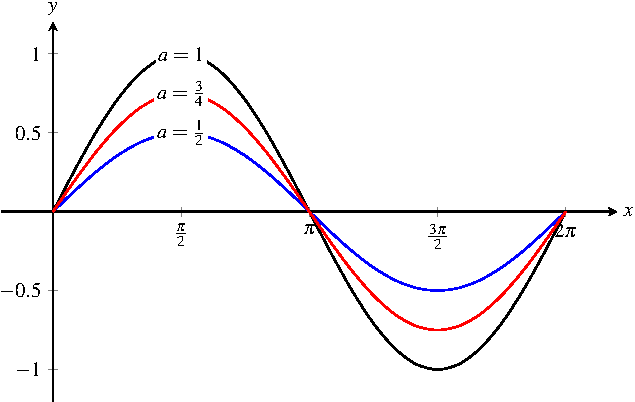
\includegraphics[scale=1.1]{image/13/sin-vertical-compress.pdf}
\caption{%%
  Graphs of the function $f(x) = a \sin x$ for
  $a = \triple{1}{\frac{3}{4}}{\frac{1}{2}}$.
}
\label{fig:trigonometric:sine_vertical_compress}
\end{figure}

\end{solution}
}{}


%%%%%%%%%%%%%%%%%%%%%%%%%%%%%%%%%%%%%%%%%%%%%%%%%%%%%%%%%%%%%%%%%%%%%%%%%%%

\section{Vertical shift of cosine function}

Let $a$ and $b$ be fixed real numbers and let $x$ be a real variable.
The cosine function can be written as
\[
f(x)
=
a \cos x + b
\]
and is graphed in \Figure{fig:trigonometric:a_cos_b} from $x = -2\pi$
to $x = 2\pi$.  The \emph{midline} of $f(x)$ is the horizontal line
$y = b$.  The \emph{amplitude} of $f(x)$ is the absolute value
$\absoluteValue{a}$.  The highest value of $f(x)$ is obtained by
adding the amplitude to the value of the midline.  Similarly, the
lowest value of $f(x)$ is obtained by subtracting the amplitude from
the value of the midline. Thus the highest value of $f(x)$ is
$b + \absoluteValue{a}$ and the lowest value of $f(x)$ is
$b - \absoluteValue{a}$.  The value $b$ of the midline is halfway
between the highest and lowest values of $f(x)$.  If $h$ is the
highest value of $f(x)$ and $\ell$ is the lowest value of $f(x)$, then
the value of the midline is the average $\frac{h + \ell}{2}$.

\begin{figure}[!htbp]
\centering
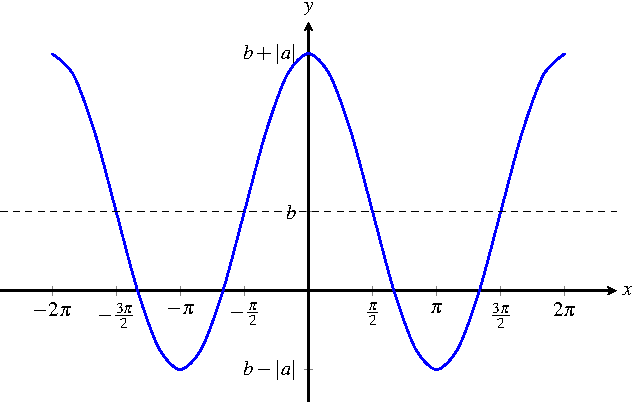
\includegraphics[scale=1.1]{image/13/a-cos-b.pdf}
\caption{%%
  A graph of the general cosine function $f(x) = a \cos x + b$ from
  $x = -2\pi$ to $x = 2\pi$.  The midline of $f(x)$ is the dashed
  horizontal line $y = b$.  The amplitude of $f(x)$ is the absolute
  value $\absoluteValue{a}$.
}
\label{fig:trigonometric:a_cos_b}
\end{figure}

Just as the value of the midline vertically shifts the graph of a sine
function, the value of the midline also vertically shifts the graph of
a cosine function.  If the value of the midline is positive,
i.e.~$b > 0$, then the graph of the cosine function will be shifted
upward.  On the other hand, if the value of the midline is negative,
i.e.~$b < 0$, the graph of the cosine function will be shifted
downward.  \Figure{fig:trigonometric:cos_vertical_shift} illustrates
the vertical shift of the graph of the cosine function.

\begin{figure}[!htbp]
\centering
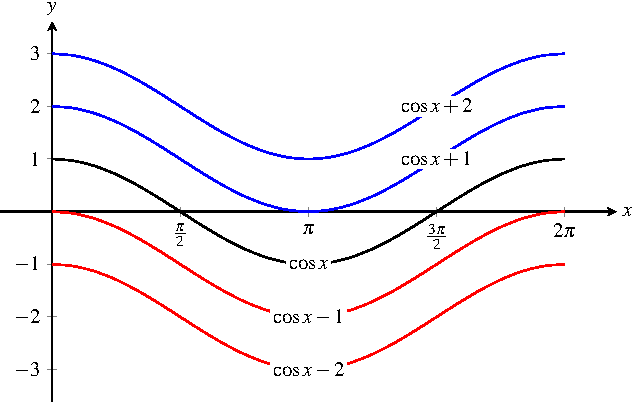
\includegraphics[scale=1.1]{image/13/cos-vertical-shift.pdf}
\caption{%%
  The value of the midline has the effect of vertically shifting the
  graph of the cosine function.
}
\label{fig:trigonometric:cos_vertical_shift}
\end{figure}

\begin{figure}[!htbp]
\centering
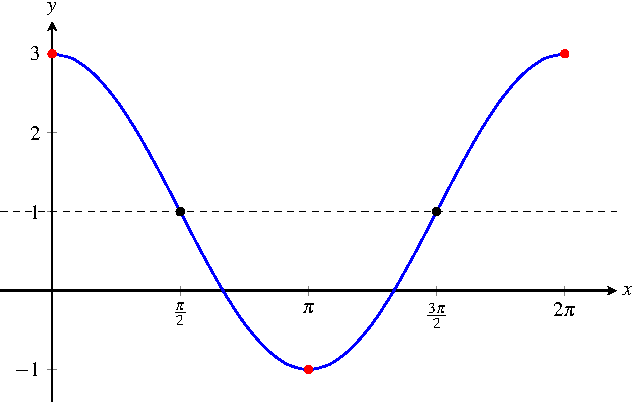
\includegraphics[scale=1.1]{image/13/2-cos-3.pdf}
\caption{%%
  A graph of the function $f(x) = 2 \cos x + 1$ from $x = 0$ to
  $x = 2\pi$.
}
\label{fig:trigonometric:2_cos_1}
\end{figure}

\begin{example}
Consider the function $f(x) = 2 \cos x + 1$.  Determine the midline
and amplitude of $f(x)$.  Calculate the highest and lowest values of
the function.  Sketch a graph of $f(x)$ from $x = 0$ to $x = 2\pi$.
\end{example}

\begin{solution}
The midline of the function $f(x)$ is $y = 1$ and the amplitude is
$2$.  The midline is shown in \Figure{fig:trigonometric:2_cos_1} as a
dashed horizontal line.  The highest value of $f(x)$ is obtained by
adding the amplitude to the value of the midline.  Thus the highest
value of $f(x)$ is $1 + 2 = 3$.  The lowest value of $f(x)$ is
obtained by subtracting the amplitude from the value of the midline.
Then the lowest value of $f(x)$ is $1 - 2 = -1$.

To sketch a graph of $f(x)$ from $x = 0$ to $x = 2\pi$, you should
first determine all points of $f(x)$ at which the graph of $f(x)$
intersects the midline $y = 1$.  That is, you want all values of $x$
such that $\cos x = 0$.  The reason is that if $\cos x = 0$ then
$f(x)$ simplifies to $f(x) = 1$, which is $y$-coordinate of the
midline.  You know that $\cos x = 0$ whenever
$x = \pair{\frac{\pi}{2}}{\frac{3\pi}{2}}$.  Then the graph of $f(x)$
intersects the midline at the points $\tuple{\frac{\pi}{2}}{1}$ and
$\tuple{\frac{3\pi}{2}}{1}$.  The points of intersection are shown in
\Figure{fig:trigonometric:2_cos_1} as black dots.

Next, you should determine the highest and lowest points of $f(x)$.
The highest value of $\cos x$ is $1$, which occurs whenever
$x = \pair{0}{2\pi}$.  Then you have
$f(0) = f(2\pi) = 2 \times 1 + 1 = 3$, which is the highest value of
$f(x)$.  Thus the highest points of $f(x)$ are $\tuple{0}{3}$ and
$\tuple{2\pi}{3}$.  Furthermore, the lowest value of $\cos x$ is $-1$,
which occurs whenever $x = \pi$.  Then you have
$f(\pi) = 2 (-1) + 1 = -1$, which is the lowest value of $f(x)$.  Thus
the lowest point of $f(x)$ is $\tuple{\pi}{-1}$.  The highest and
lowest points of $f(x)$ are shown in
\Figure{fig:trigonometric:2_cos_1} as red dots.

Finally, draw a wave through the five points above to obtain the graph
shown in \Figure{fig:trigonometric:2_cos_1}.
\end{solution}

\begin{exercise}
Consider the function $f(x) = \frac{3}{2} \cos x - 1$.  Determine the
midline and amplitude of the function.  Calculate the highest and
lowest values of $f(x)$.  Sketch a graph of $f(x)$ from $x = 0$ to
$x = 2\pi$.
\end{exercise}

\ifbool{showSolution}{
\begin{solution}
The function $f(x)$ has a midline of $y = -1$ and an amplitude of
$3/2$.  \Figure{fig:trigonometric:3half_cos_minus1} shows the midline
as a dashed horizontal line.  The highest value of $f(x)$ is obtained
by adding the amplitude to the value of the midline.  That is, the
highest value of $f(x)$ is
%%
\begin{align*}
-1 + \frac{3}{2}
&=
\frac{-2}{2} + \frac{3}{2} \\[4pt]
&=
\frac{-2 + 3}{2} \\[4pt]
&=
\frac{1}{2}.
\end{align*}
%%
The lowest value of $f(x)$ is obtained by subtracting the amplitude
from the value of the midline.  In other words, the lowest value of
$f(x)$ is
%%
\begin{align*}
-1 - \frac{3}{2}
&=
\frac{-2}{2} - \frac{3}{2} \\[4pt]
&=
\frac{-2 - 3}{2} \\[4pt]
&=
-\frac{5}{2}.
\end{align*}

\begin{figure}[!htbp]
\centering
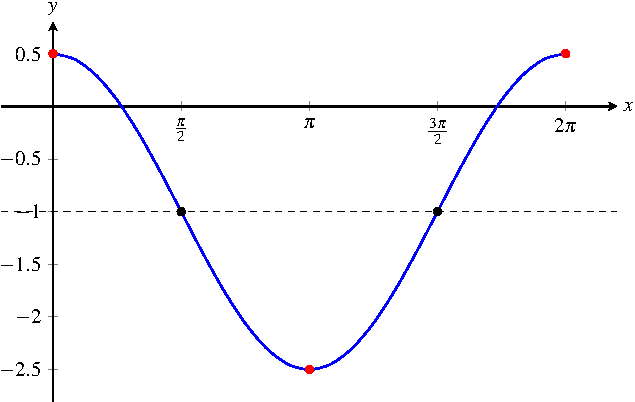
\includegraphics[scale=1.1]{image/13/3half-cos-minus1.pdf}
\caption{%%
  A graph of the function $f(x) = \frac{3}{2} \cos x - 1$ from $x = 0$
  to $x = 2\pi$.
}
\label{fig:trigonometric:3half_cos_minus1}
\end{figure}

To sketch a graph of $f(x)$ from $x = 0$ to $x = 2\pi$, first you
should determine all points at which the graph of $f(x)$ intersects
the midline.  This is the same as determining all values of $x$ such
that $\cos x = 0$.  You know that $\cos x = 0$ whenever
$x = \pair{\frac{\pi}{2}}{\frac{3\pi}{2}}$ and so you have
$f(\pi/2) = f(3\pi/2) = \frac{3}{2} \times 0 - 1 = -1$.  Thus the
graph of $f(x)$ intersects the midline at the points
$\tuple{\frac{\pi}{2}}{-1}$ and $\tuple{\frac{3\pi}{2}}{-1}$.  The
points of intersection are shown in
\Figure{fig:trigonometric:3half_cos_minus1} as black dots.

Next, you determine the highest and lowest points of $f(x)$.  The
highest value of $\cos x$ is $1$, which occurs whenever
$x = \pair{0}{2\pi}$.  Then you have
$f(0) = f(2\pi) = \frac{3}{2} \times 1 - 1 = \frac{1}{2}$.  The lowest
value of $\cos x$ is $-1$, which occurs whenever $x = \pi$.  Then you
have $f(\pi) = \frac{3}{2} (-1) - 1 = -\frac{5}{2}$.  In other words,
the highest points of $f(x)$ are $\tuple{0}{\frac{1}{2}}$ and
$\tuple{2\pi}{\frac{1}{2}}$.  The lowest point of $f(x)$ is
$\tuple{\pi}{-\frac{5}{2}}$.  The highest and lowest points are shown
in \Figure{fig:trigonometric:3half_cos_minus1} as red dots.

Finally, draw a wave through the above five points and you obtain the
graph in \Figure{fig:trigonometric:3half_cos_minus1}.
\end{solution}
}{}

\begin{exercise}
Consider the function $f(x) = -4 \cos x + 3$.  Determine the midline
and amplitude of $f(x)$.  Calculate the highest and lowest values of
the function.  Draw a graph of $f(x)$ from $x = 0$ to $x = 2\pi$.
\end{exercise}

\ifbool{showSolution}{
\begin{solution}
The midline of the function $f(x)$ is $y = 3$, which is shown in
\Figure{fig:trigonometric:minus4_cos_3} as a dashed horizontal line.
The amplitude of the function is the absolute value
$\absoluteValue{-4} = 4$.  The highest value of $f(x)$ is obtained by
adding the amplitude to the value of the midline.  Thus the highest
value of $f(x)$ is $3 + 4 = 7$.  The lowest value of $f(x)$ is
obtained by subtracting the amplitude from the value of the midline.
That is, the lowest value of $f(x)$ is $3 - 4 = -1$.

\begin{figure}[!htbp]
\centering
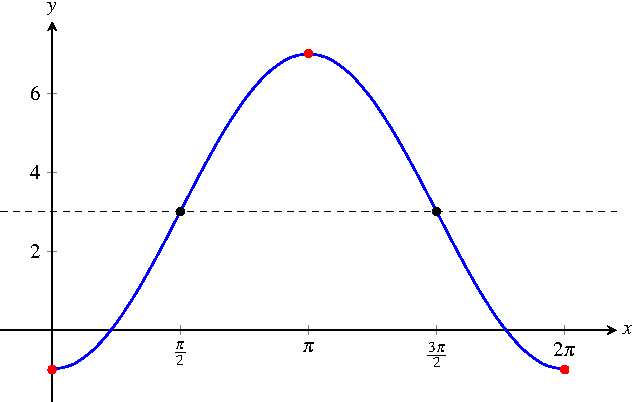
\includegraphics[scale=1.1]{image/13/minus4-cos-3.pdf}
\caption{%%
  A graph of the function $f(x) = -4 \cos x + 3$ from $x = 0$ to
  $x = 2\pi$.
}
\label{fig:trigonometric:minus4_cos_3}
\end{figure}

To draw a graph of $f(x)$ from $x = 0$ to $x = 2\pi$, you should first
determine all points at which the graph of $f(x)$ intersects the
midline.  This occurs for all values of $x$ such that $\cos x = 0$
because if $\cos x = 0$ then the function $f(x)$ simplifies to
$f(x) = 3$, which is the value of the midline.  You know that
$\cos x = 0$ whenever $x = \pair{\frac{\pi}{2}}{\frac{3\pi}{2}}$.
Then you have $f(\pi/2) = f(3\pi/2) = -4 \times 0 + 3 = 3$ and so the
graph of $f(x)$ intersects the midline at the points
$\tuple{\frac{\pi}{2}}{3}$ and $\tuple{\frac{3\pi}{2}}{3}$.  The
points of intersection are shown in
\Figure{fig:trigonometric:minus4_cos_3} as black dots.

Next, you should determine the highest and lowest points of $f(x)$.
Note that the highest value of $\cos x$ is $1$, which occurs whenever
$x = \pair{0}{2\pi}$.  Then you have
$f(0) = f(2\pi) = -4 \times 1 + 3 = -1$, which is the lowest value of
$f(x)$.  Thus the lowest points of $f(x)$ are $\tuple{0}{-1}$ and
$\tuple{2\pi}{-1}$.  Furthermore, the lowest value of $\cos x$ is
$-1$, which occurs whenever $x = \pi$.  Then you have
$f(\pi) = -4 (-1) + 3 = 7$, which is the highest value of $f(x)$.  In
other words, the highest point of $f(x)$ is $\tuple{\pi}{7}$.  The
highest and lowest points of $f(x)$ are shown in
\Figure{fig:trigonometric:minus4_cos_3} as red dots.

Finally, draw a wave through the above five points and you obtain the
graph shown in \Figure{fig:trigonometric:minus4_cos_3}.
\end{solution}
}{}

\begin{figure}[!htbp]
\centering
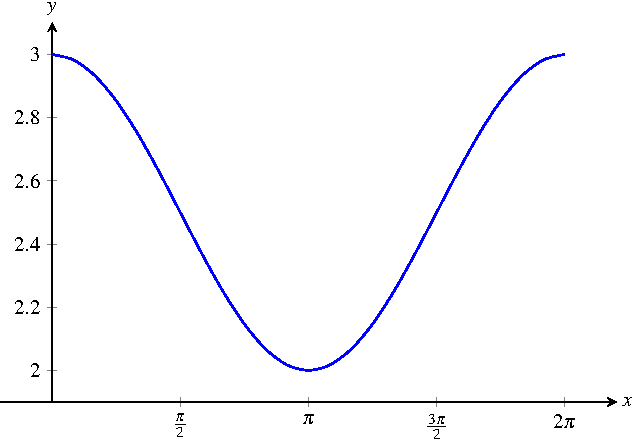
\includegraphics[scale=1.1]{image/13/half-cos-5half.pdf}
\caption{%%
  A graph of a cosine function of the form $f(x) = a \cos x + b$ from
  $x = 0$ to $x = 2\pi$.
}
\label{fig:trigonometric:half_cos_5half}
\end{figure}

\begin{exercise}
\Figure{fig:trigonometric:half_cos_5half} shows a graph of a cosine
function, whose midline is $y = 5/2$.  The function has $\tuple{0}{3}$
as one of its highest points.  If the function is of the form
$f(x) = a \cos x + b$, determine the values of $a$ and $b$.
\end{exercise}

\ifbool{showSolution}{
\begin{solution}
Since the midline is $y = 5/2$, then you have $b = 5/2$.  To get the
highest value of the function, you add the amplitude to the value of
the midline.  If the amplitude is $a$, then you have the equation
$\frac{5}{2} + a = 3$.  Solving the latter equation for $a$ shows that
%%
\begin{align*}
a
&=
3 - \frac{5}{2} \\[4pt]
&=
\frac{6}{2} - \frac{5}{2} \\[4pt]
&=
\frac{6 - 5}{2} \\[4pt]
&=
\frac{1}{2}.
\end{align*}
%%
In other words, the amplitude is $1/2$.  Thus
\Figure{fig:trigonometric:half_cos_5half} shows a graph of the
function $f(x) = \frac{1}{2} \cos x + \frac{5}{2}$.
\end{solution}
}{}

\begin{exercise}
A cosine function $f(x) = a \cos x + b$ has $\tuple{0}{\frac{11}{2}}$
and $\tuple{\pi}{\frac{1}{2}}$ as some of its highest and lowest
points, respectively.  Determine the amplitude and midline of $f(x)$.
Sketch a graph of $f(x)$ from $x = 0$ to $x = 2\pi$.
\end{exercise}

\ifbool{showSolution}{
\begin{solution}
The highest and lowest values of $f(x)$ are $\frac{11}{2}$ and
$\frac{1}{2}$, respectively.  The value of the midline of $f(x)$ is
the average of the highest and lowest values of $f(x)$.  Thus the
midline of $f(x)$ is
%%
\begin{align*}
y
&=
\frac{1}{2} \parenthesis*{\frac{11}{2} + \frac{1}{2}} \\[4pt]
&=
\frac{1}{2} \parenthesis*{\frac{11 + 1}{2}} \\[4pt]
&=
\frac{1}{2} \times 6 \\[4pt]
&=
3.
\end{align*}
%%
The amplitude of $f(x)$ is the difference between the highest value of
$f(x)$ and the value of the midline.  The amplitude can also be
calculated as the difference between the value of the midline and the
lowest value of $f(x)$.  That is, the amplitude of $f(x)$ is
%%
\begin{align*}
\frac{11}{2} - 3
&=
\frac{11}{2} - \frac{6}{2} \\[4pt]
&=
\frac{11 - 6}{2} \\[4pt]
&=
\frac{5}{2}.
\end{align*}
%%
Then the function $f(x)$ can be written as
$f(x) = \frac{5}{2} \cos x + 3$, which is graphed in
\Figure{fig:trigonometric:5half_cos_3}.

\begin{figure}[!htbp]
\centering
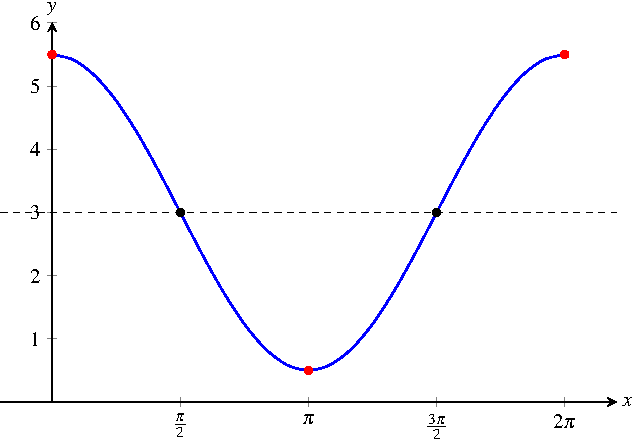
\includegraphics[scale=1.1]{image/13/5half-cos-3.pdf}
\caption{%%
  A graph of the function $f(x) = \frac{5}{2} \cos x + 3$ from $x = 0$
  to $x = 2\pi$.
}
\label{fig:trigonometric:5half_cos_3}
\end{figure}

\end{solution}
}{}

\begin{exercise}
Consider the function $f(x) = a \cos x$.  Graph the function for
$a = \triple{1}{\frac{3}{2}}{2}$.  Also graph the function for
$a = \triple{1}{\frac{1}{2}}{\frac{3}{4}}$.  Describe the effect of
the value of the amplitude on the graph of the cosine function.
\end{exercise}

\ifbool{showSolution}{
\begin{solution}
\Figures{fig:trigonometric:cos_vertical_stretch}{fig:trigonometric:cos_vertical_compress}
show graphs of the function $f(x) = a \cos x$ for
$a = \triple{1}{\frac{3}{2}}{2}$ and for
$a = \triple{1}{\frac{1}{2}}{\frac{3}{4}}$.  When the amplitude is
$a > 1$, the graph of the cosine function is stretched vertically.
However, when the amplitude is $0 < a < 1$, the graph of the cosine
function is compressed vertically.  That is, the value of the
amplitude has the effect of stretching or compressing in the vertical
direction the graph of the cosine function.

\begin{figure}[!htbp]
\centering
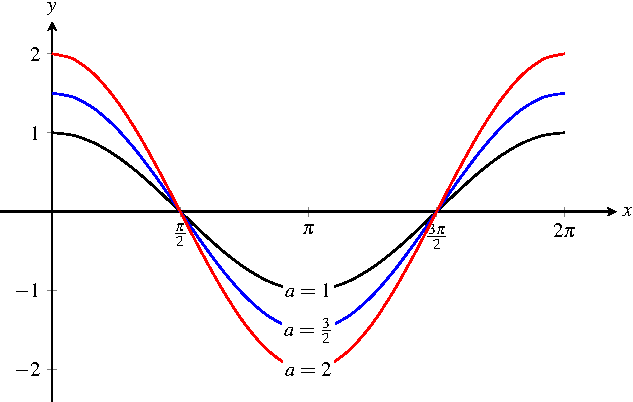
\includegraphics[scale=1.1]{image/13/cos-vertical-stretch.pdf}
\caption{%%
  Graphs of the function $f(x) = a \cos x$ for
  $a = \triple{1}{\frac{3}{2}}{2}$.
}
\label{fig:trigonometric:cos_vertical_stretch}
\end{figure}

\begin{figure}[!htbp]
\centering
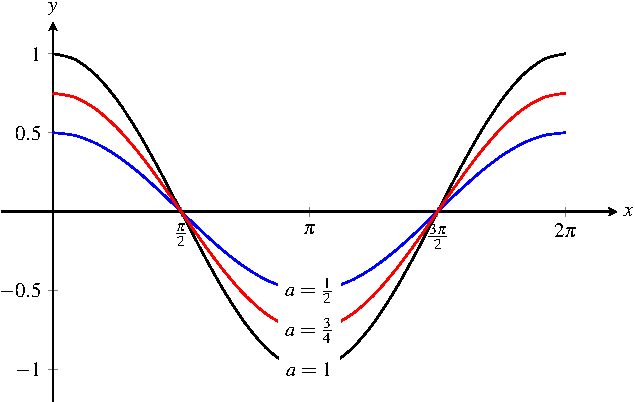
\includegraphics[scale=1.1]{image/13/cos-vertical-compress.pdf}
\caption{%%
  Graphs of the function $f(x) = a \cos x$ for
  $a = \triple{1}{\frac{1}{2}}{\frac{3}{4}}$.
}
\label{fig:trigonometric:cos_vertical_compress}
\end{figure}

\end{solution}
}{}


%%%%%%%%%%%%%%%%%%%%%%%%%%%%%%%%%%%%%%%%%%%%%%%%%%%%%%%%%%%%%%%%%%%%%%%%%%%

\section{Period and frequency}

Let $\triple{a}{b}{c}$ be fixed real numbers and let $x$ be a real
variable.  Consider the sine and cosine functions of the form
\[
f(x)
=
a \sin(cx) + b
%%
\qquad
\text{and}
\qquad
%%
g(x)
=
a \cos(cx) + b.
\]
You already know that the amplitude is the absolute value
$\absoluteValue{a}$ and the midline is $y = b$.  What effect does the
value of $c$ have on the graph of $f(x)$ and $g(x)$?  To understand
how the value of $c$ affects the graph of the sine and cosine
functions, consider the simpler functions $F(x) = \sin(cx)$ and
$G(x) = \cos(cx)$.
\Figure{subfig:trigonometric:sine_horizontal_stretch} shows graphs of
$F(x)$ for $c = \triple{1}{\frac{3}{4}}{\frac{1}{2}}$ and
\Figure{subfig:trigonometric:sine_horizontal_compress} shows some
graphs of $F(x)$ for $c = \triple{1}{\frac{3}{2}}{2}$.  The figures
show that when $0 < c < 1$ the value of $c$ stretches the graph of the
sine function along the horizontal direction.  However, when $c > 1$
the value of $c$ horizontally compresses the graph of the sine
function.  Thus the value of $c > 0$ has the effect of stretching or
compressing along the horizontal axis the graph of the sine function.

\begin{figure}[!htbp]
\centering
\subfigure[]{
  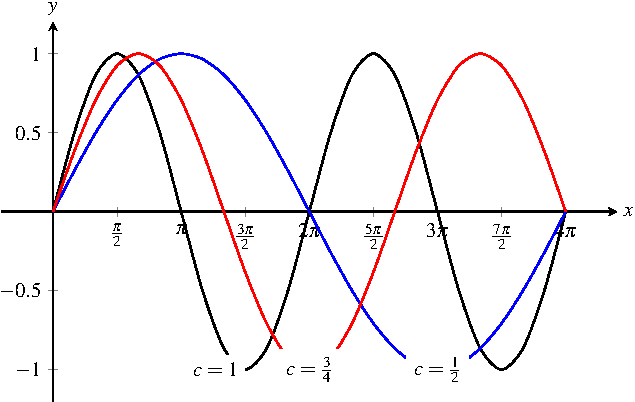
\includegraphics[scale=1.1]{image/13/sin-horizontal-stretch.pdf}
  \label{subfig:trigonometric:sine_horizontal_stretch}
}
%%
%%
\subfigure[]{
  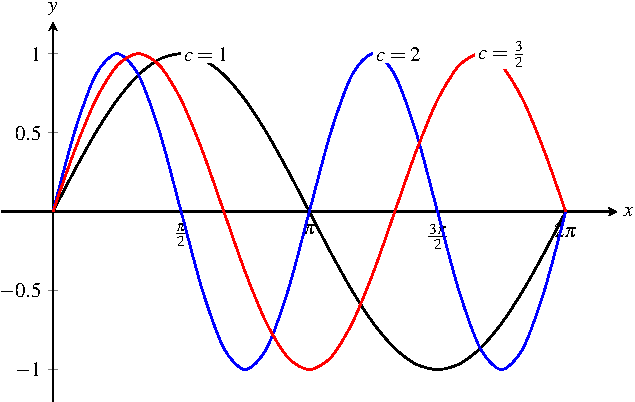
\includegraphics[scale=1.1]{image/13/sin-horizontal-compress.pdf}
  \label{subfig:trigonometric:sine_horizontal_compress}
}
\caption{%%
  Various graphs of the sine function $F(x) = \sin(cx)$ for
  (a)~$c = \triple{1}{\frac{3}{4}}{\frac{1}{2}}$ and
  (b)~$c = \triple{1}{\frac{3}{2}}{2}$.
}
\label{fig:trigonometric:sine_horizontal_stretch_compress}
\end{figure}

\begin{exercise}
Graph the cosine function $G(x) = \cos(cx)$ for
$c = \triple{1}{\frac{3}{4}}{\frac{1}{2}}$.  Also graph $G(x)$ for
$c = \triple{1}{\frac{4}{3}}{2}$.  If $c > 0$, describe the effect of
the value of $c$ on the graph of the cosine function.
\end{exercise}

\ifbool{showSolution}{
\begin{solution}
\Figures{subfig:trigonometric:cosine_horizontal_stretch}{subfig:trigonometric:cosine_horizontal_compress}
show various graphs of the cosine function $G(x) = \cos(cx)$ for
$c = \triple{1}{\frac{3}{4}}{\frac{1}{2}}$ and
$c = \triple{1}{\frac{4}{3}}{2}$.  As can be seen from the figures,
when $0 < c < 1$ the value of $c$ effectively stretches along the
horizontal direction the graph of the cosine function.  However, when
$c > 1$ the value of $c$ compresses along the horizontal direction the
graph of the cosine function.  In effect, the value of $c > 0$
stretches or compresses the graph of the cosine function along the
horizontal axis.

\begin{figure}[!htbp]
\centering
\subfigure[]{
  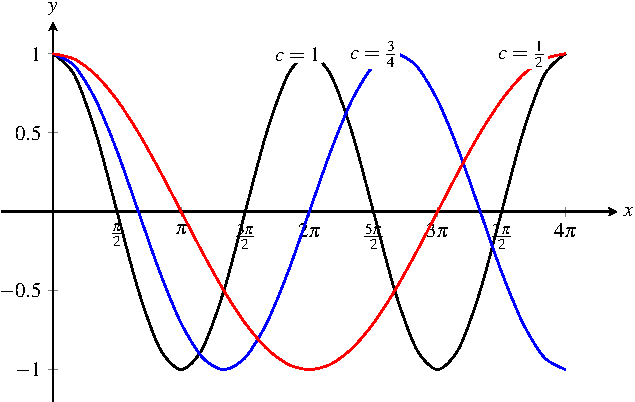
\includegraphics[scale=1.1]{image/13/cos-horizontal-stretch.pdf}
  \label{subfig:trigonometric:cosine_horizontal_stretch}
}
%%
%%
\subfigure[]{
  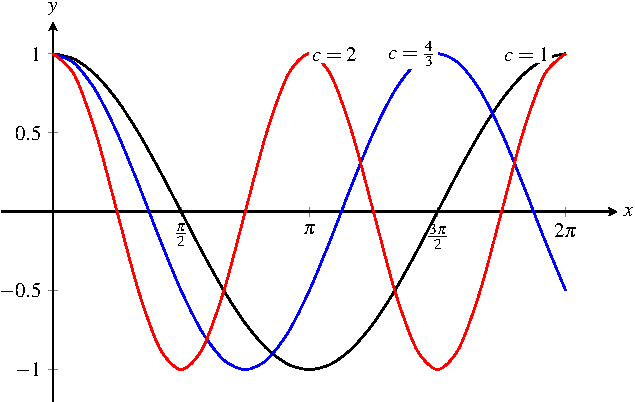
\includegraphics[scale=1.1]{image/13/cos-horizontal-compress.pdf}
  \label{subfig:trigonometric:cosine_horizontal_compress}
}
\caption{%%
  Various graphs of the cosine function $G(x) = \cos(cx)$ for
  (a)~$c = \triple{1}{\frac{3}{4}}{\frac{1}{2}}$ and
  (b)~$c = \triple{1}{\frac{4}{3}}{2}$.
}
\label{fig:trigonometric:cosine_horizontal_stretch_compress}
\end{figure}

\end{solution}
}{}

\end{document}
